% !TEX root =  ../main_manuscript.tex 
\section{Results}
\subsection{General Results}
In PRIAS, the probability of experiencing reclassification within the first five and ten years was 33\% and 42\%, respectively (cumulative-risk plot in Appendix A). That is, ideally more than 50\% of the patients may not require any biopsy in the first ten years.

\subsection{Joint Model Results} 
For every ten years increase in a patient age at the time diagnosis, the adjusted hazard ratio of reclassification is 1.45~(95\%CI:~1.30--1.63). When fitted PSA value (log scale) increases from 2.36 (25-th percentile of fitted PSA) to 3.07 (75-th percentile of fitted PSA), the adjusted hazard ratio of reclassification is 0.99~(95\%CI:~0.89--1.11). When estimated instantaneous PSA (log scale) velocity increases from -0.09 (25-th percentile of estimated velocity) to 0.31 (75-th percentile of estimated velocity), the adjusted hazard ratio of reclassification is 2.47~(95\%CI:~1.93--2.99). Hence, the instantaneous PSA (log scale) velocity is a stronger predictor for hazard of reclassification than the PSA value (log scale). Detailed parameter estimates are in Appendix~A.4.

\subsection{Validation Results}
Using the joint model fitted to the PRIAS dataset we made risk predictions for GS7 in real PRIAS patients. As shown in Figure 4 of Appendix B, these risk estimates become more accurate as more data is gathered over follow-up. To check the accuracy of these risk predictions, we calculated the time dependent area under the receiver operating characteristic curves (AUC) as a measure of discrimination, and the root mean squared prediction error (RMSPE) as a measure of calibration. These are shown in Figure~\ref{fig:auc_pe}. For predictions within PRIAS (internal validation), the time-dependent AUC was between 0.62 and 0.69, and RMSPE between 0.23 and 0.37 over the whole follow-up period. For validation in external cohorts, the AUC was similar to the AUC of PRIAS for all cohorts during the first three years of follow-up. The RMPSE however differed much more during the same period. The AS cohorts closest to PRIAS in terms of RMSPE were Johns Hopkins Active Surveillance and Memorial Sloan Kettering Cancer Center Active Surveillance. Detailed AUC and RMSPE results for all cohorts with 95\% bootstrapped confidence intervals are presented in Table 6 to Table 11 of Appendix B.

\begin{figure}
\centerline{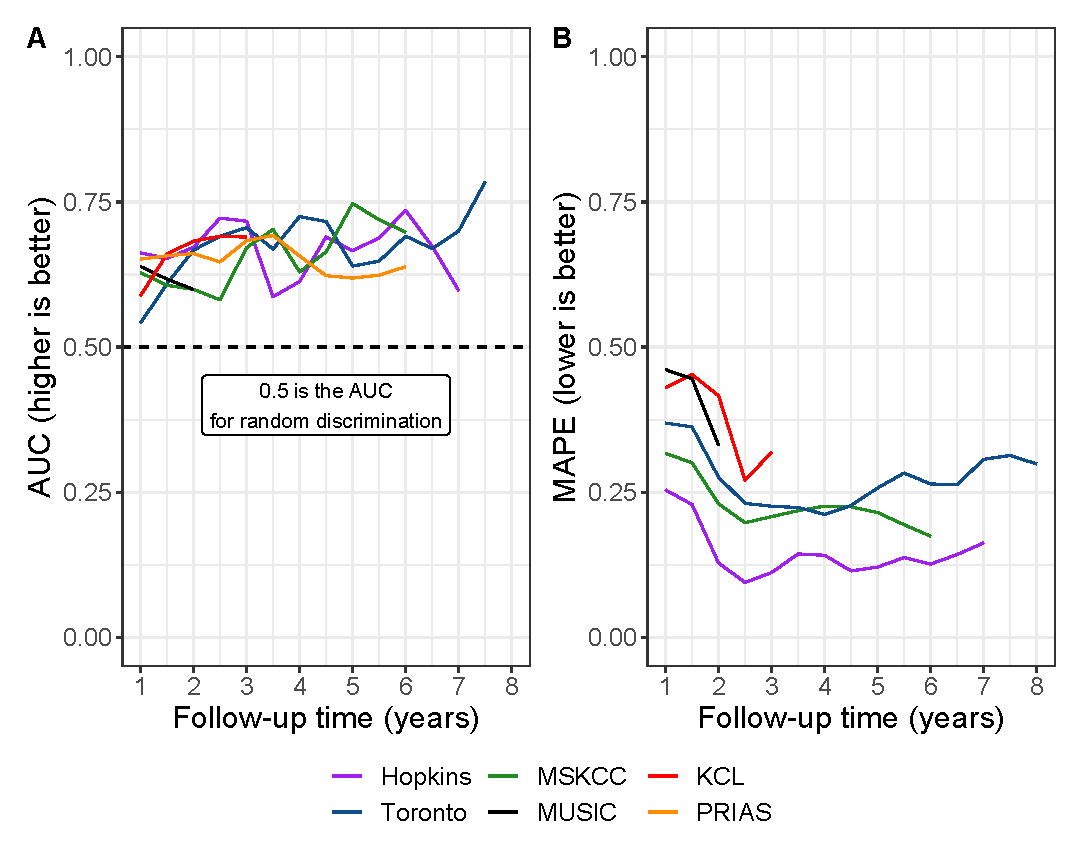
\includegraphics[width=\columnwidth]{images/auc_pe.eps}}
\caption{\textbf{Validation of predictions of Gleason $\geq$ 7 (GS7)}. In \textbf{Panel~A} we can see that the time dependent area under the receiver operating characteristic curve or AUC (measure of discrimination) is above 0.5 in PRIAS (internal validation), and in Toronto, JHAS, MSKCC, KCL, and MUSIC AS cohorts (external validation). In \textbf{Panel~B} we can see that the time dependent root mean squared prediction error or RMSPE (measure of calibration) is similar for PRIAS, and JHAS and Toronto cohorts. The bootstrapped 95\% confidence interval for these estimates are presented in Table 6 to Table 11 of Appendix B. Full names of Cohorts are \textit{PRIAS}: Prostate Cancer International Active Surveillance, \textit{Toronto}: University of Toronto Active Surveillance, \textit{JHAS}: Johns Hopkins Active Surveillance, \textit{MSKCC}: Memorial Sloan Kettering Cancer Center Active Surveillance, \textit{KCL}: King's College London Active Surveillance, \textit{MUSIC}: Michigan Urological Surgery Improvement Collaborative Active Surveillance.}
\label{fig:auc_pe}
\end{figure}

\subsection{Personalized Schedule Results}
Using the risk predictions for GS7, we developed personalized schedules of biopsy for real PRIAS patients. We maintained a minimum gap of one year between biopsies as advised by the PRIAS protocol. In addition, we scheduled biopsies only for the first ten years follow-up because of limited follow-up period of the training dataset PRIAS. A compulsory biopsy was done scheduled year ten of follow-up in all schedules for meaningful comparison of their expected delays in detection of GS7. Various personalized and fixed biopsy schedules for demo patients are shown in Figure \ref{fig:demo_pat1} and Appendix C's Figure 6, 7, 8 and 9. The biopsies denoted by `B' show that personalized schedules schedule fewer biopsies than fixed schedules. At the same time the expected time delay in detection of GS7 is less than an year for personalized schedules. We have implemented this approach in a web-application (\url{https://emcbiostatistics.shinyapps.io/prias_biopsy_recommender/}, and Appendix D) for practical use.